\mytitle{Field-theory approach to quantum many-body systems}
Yesterday, we have considered the Hamiltonian, which can be transformed into the Lagrangian form as
\begin{equation}
\mathcal{L}=\frac{1}{2\pi k}(\partial_\mu \phi)^2
\end{equation}
which is same with the Lagrangian of vibration of the string, which is actually a gapless system. But in the real system, most of the systems are gapped, and the gaplessness comes out on a critical point. Therefore we often say the gapless point as "critical point". Therefore, in some sense, the gaplessness of spin $1/2$ chain is rather surprising then the gaplessness of spin $1$ chain.

Now we come back to the original model, which is the spin chain model. In this model, $S_j^\alpha$ is defined on lattice points, whose lattice constant is $a$. Then, from previous argument,
\begin{equation}
S_j^z=-S+n_j=-S+\int_{(j-\frac{1}{2})a}^{(j+\frac{1}{2})a}\rho(x)dx
\end{equation}
where
\begin{equation}
\rho(x)=\left[\rho_0-\frac{1}{\pi}\partial_x\phi\right]\sum_{p\in \mathbb{Z}}e^{2ip[\pi\rho_0 x-\phi(x)]}
\end{equation}
Now $p=0$ term gives the term
\begin{equation}
\rho_0 a-\frac{1}{\pi}[\phi((j+\frac{1}{2})a)-\phi((j-\frac{1}{2})a)]
\end{equation}
What we get when $p\neq 0$? Considering $\phi(x)$ varying very linearly and slowly, we may consider $\partial_x\phi$ and $\phi(x)$ be a small constant when we take integral. Then we get
\begin{equation}
\frac{1}{2\pi p i}\left[e^{2p i\left[\pi \rho_0 \left(j+\frac{1}{2}\right)a-\phi\left(\left(j+\frac{1}{2}\right)a\right)\right]}-e^{2p i\left[\pi \rho_0 \left(j-\frac{1}{2}\right)a-\phi\left(\left(j-\frac{1}{2}\right)a\right)\right]}\right]
\end{equation}
Now notice that the ground state of spin-$S$ antiferromagnetic chain must have $\langle S_j^z\rangle=0$, considereing N{\'e}el state. This implies $\langle n_j\rangle=S$, i. e. $\rho_0 a=S$. Here the spin quantum number enters. Putting this value, we write $p\neq 0$ term as
\begin{equation}
\frac{1}{2\pi p i}\left[e^{2p i\left[\pi S \left(j+\frac{1}{2}\right)-\phi\left(\left(j+\frac{1}{2}\right)a\right)\right]}-e^{2p i\left[\pi S \left(j-\frac{1}{2}\right)-\phi\left(\left(j-\frac{1}{2}\right)a\right)\right]}\right]
\end{equation}

From this, we can calculate the $S_j^z$ operator using $\phi(x)$ field. We have two possible cases: $S\in \mathbb{Z}$ and $S\in \mathbb{Z}+\frac{1}{2}$, which gives quite different results: if $S\in \mathbb{Z}$, then
\begin{equation}
S_j^z=A\partial_x \phi\left[1+\sum_{p\geq 0}C_p\cos(2p\phi(x))\right]
\end{equation}
and if $S\in \mathbb{Z}+\frac{1}{2}$, then
\begin{align*}
S_j^z=B\partial_x \phi&\left[1+\sum_{p=2,4,6,\cdots}D_p\cos(2p\phi(x))\right.\\
&+(-1)^j\left.\sum_{p=1,3,5,\cdots}D_p\sin(2p\phi(x))\right]\numberthis
\end{align*}
where the $\mathcal{O}((\partial_x\phi)^2)$ terms are ignored here.

Using this, we can represent the operator $S_j^zS_{j+1}^z$. Here, it is good method to use the \textbf{operator product expansion}, which is the expansion of the product of two operators in short distance to the expansion by a single point operator.\marginnote{This job can be done by writing down the field into creation and annihilation operators, or by using the Wick's theorem.} Then we get
\begin{equation}
S_j^z S_{j+1}^z\sim \underbrace{A+B(\partial_x\phi)^2}_{\mathcal{H}_{\textrm{TLL}}}+\underbrace{\sum_{p\geq 1}C_p \cos(2p\phi(x))+\cdots}_{\mathcal{H}'}
\end{equation}
where $S\in \mathbb{Z}$ and
\begin{align*}
S_j^{z} S_{j+1}^z\sim \underbrace{A+B(\partial_x\phi)^2}_{\mathcal{H}_{\textrm{TLL}}}&+\underbrace{(-1)^j\sum_{p=1,3,5,\cdots}C_p\sin(2p\phi(x))}_{\textrm{Vanishes by} \sum_j}\\
&+\underbrace{\sum_{p=2,4,6,\cdots}C_p\sin(2p\phi(x))+\cdots}_{\mathcal{H}'}
\end{align*}
where $S\in \mathbb{Z}+\frac{1}{2}$. Here $\mathcal{H}_{\textrm{TLL}}$ is the Tomonaga-Luttinger liquid Hamiltonian.

Now the Hamiltonian-included term $\cos(2p\phi(x))$ can be written as $\frac{1}{2}\left[e^{2ip\phi(x)}+e^{-2ip\phi(x)}\right]$. Thus we are curious about the fact that what $e^{2ip\phi(x)}$ does on the state. To do this, first we know
\begin{equation}
[\phi(x),\theta(x')]=-\frac{i\pi}{2}\sgn(x-x')
\end{equation}
thus
\begin{equation}
[e^{2ip\phi(x)},\theta(x')]=\pi p\sgn(x-x')e^{2ip\phi(x)}
\end{equation}
Now suppose $e^{2ip\phi(y)}$ is applied on $|\theta(x)=0\rangle$ state. Then
\begin{equation}
\theta(x)\left[e^{2ip\theta(y)}|\theta(x)=0\rangle\right]=-\pi p \sgn(y-x)[e^{2ip\theta(y)}|\theta=0\rangle]
\end{equation}
This means we get the state whose phase factor $\theta(x)$ changes oppositely with the boundary point $y$. Thus by the time evolution, we get the vortex-like structure.
\begin{figure}[h!]
\center
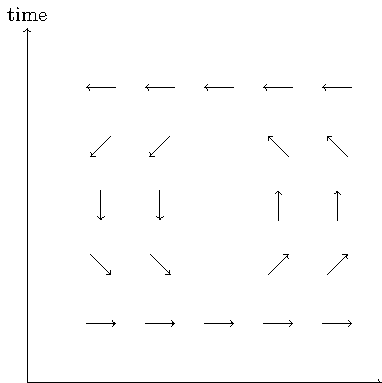
\includegraphics[width=0.5\textwidth]{vortex.pdf}
\caption{The vortex-like structure appearing when $p=1$}
\end{figure}

Notice that this vortex-like structure only appears when $p=1$, thus for $S\in \mathbb{Z}+\frac{1}{2}$ case, there is no such a vortex structure.

Now come back to the Lagrangian
\begin{equation}
\mathcal{L}=\mathcal{L}_{\textrm{TLL}}+\sum_p \lambda_p\cos(2p\phi)
\end{equation}
If we calculate the correlation of interaction, then we get
\begin{equation}
\langle \cos(2p\phi(x))\cos(2p\phi(y))\rangle_{\textrm{TLL}}\sim |x-y|^{-2p^2\kappa}
\end{equation}
where $\kappa$ is the Luttinger parameter which is determined by the interaction. This is because the scaling parameter of $e^{\pm 2ip\phi}$ is $p^2\kappa$. Thus, if we calculate the Renormalization of the action
\begin{equation}
S=\int dxd\tau \mathcal{L}
\end{equation}
then the $\lambda_p$ becomes $\lambda_p l^{2-p^2\kappa}$. Here 2 is the spacetime dimension. Thus, if $p^2\kappa>2$ then $\lambda_p\rightarrow 0$, which is called \textbf{irrelevant}, and if $p^2\kappa<2$ then $\lambda_p\rightarrow \infty$, which is called \textbf{relevant}.

Now consider the Heisenberg antiferromagnetic chain, which is $\Delta=1$ case for $XXZ$ model. This system has $\kappa=\frac{1}{2}$,\marginnote{The Tomonaga-Luttinger liquid with $k=\frac{1}{2}$ is equivalent to the $SU(2)$ Wess-Zumino-Witten model with level $1$.} Now if $p=1$ then $p^2 \kappa=\frac{1}{2}<2$, thus $e^{2i\phi}$ is relevant and $\cos(2\phi)$ term dominates. Therefore the lowest value of Lagrangian is fixed at $\phi=\pi$, which implies the gapped system. However, if $p=2$, then $p^2\kappa=2$, which is the marginal case: $e^{4i\phi}$ can be relevant or not. If it is relevant, then the system is gapped; if it is irrelevant, then the system is gapless.\marginnote{However, by using the Lieb-Schultz-Mattis theorem, we can show that the $p=2$ case, i.e. $S\in \mathbb{Z}+\frac{1}{2}$ case, is gapless.}

Until here, we only thought the operators $e^{2ip\phi}$ terms, but $e^{iq\theta}$ terms also exists. To satisfy the boundary condition $\theta\sim \theta+2\pi$, we must have $q\in \mathbb{Z}$. In this case, the scaling dimension of $e^{iq\theta}$ is $\frac{q^2}{4\kappa}$, which can be relevant. However, if the original system has $U(1)$ symmetry, i.e. conservation of $S^z$, then $e^{iq\theta}$ term cannot appear because it breaks $U(1)$ symmetry.

We can play the similar argument for $\phi$ field. Recall
\begin{equation}
\phi_l(x)=2\pi\rho_0 x-2\phi(x)
\end{equation}
then
\begin{equation}
\phi_l(x+\delta x)=2\pi \rho_0(x+\delta x)-2\phi(x+\delta x)
\end{equation}
Now by translation $x\mapsto x+\delta x$ if $\phi_l(x)$ changes to $\phi_l(x+\delta x)$, then we get
\begin{equation}
\phi(x)\mapsto \phi(x)+\phi'(x)\delta x-\pi \rho_0\delta x=\phi(x)-\pi \rho_0\delta x
\end{equation}
where $\phi'\rightarrow 0$.

From the boundary condition of $\phi_l$, $\phi_l\sim \phi_l+2\pi$, thus $\phi\sim \phi+\pi$. Now if we consider the operator $e^{2ip\phi}$, then this is well defined only if $p\in \mathbb{Z}$.

Now we need to consider the lattice translation symmetry, $x\mapsto x+a$. Then $\phi\mapsto \phi-\pi\rho_0 a$. Now using $\rho_0=S/a$ for the ground state of spin chain, $\phi\mapsto \phi-\pi S$, and $e^{2ip\phi}\mapsto e^{2ip\phi}e^{2\pi i S}$. Thus, $e^{2ip\phi}$ is translational invariant if $S\in \mathbb{Z}$ or $p\in 2\mathbb{Z}$, and not translational invariant if $S\in\mathbb{Z}+\frac{1}{2}$ and $p\in 2\mathbb{Z}+1$. This result can be compared with the allowed interaction terms calculated above. Furthermore, this result also implies that if translational symmetry is broken, then $e^{2ip\phi}$ with odd $p$ are allowed, which may open the gap. the good example is the following Hamiltonian:
\begin{equation}
\mathcal{H}=J\sum_j \left[1+(-1)^j\delta\right](S_j^x S_{j+1}^x+S_j^y S_{j+1}^y+S_j^z S_{j+1}^z)
\end{equation}
The gap of this Hamiltonian with $S\in \mathbb{Z}+\frac{1}{2}$ and $S\in\mathbb{Z}$ are following, which shows that breaking the translational symmetry opens the gap.
\begin{figure}[h!]
\center
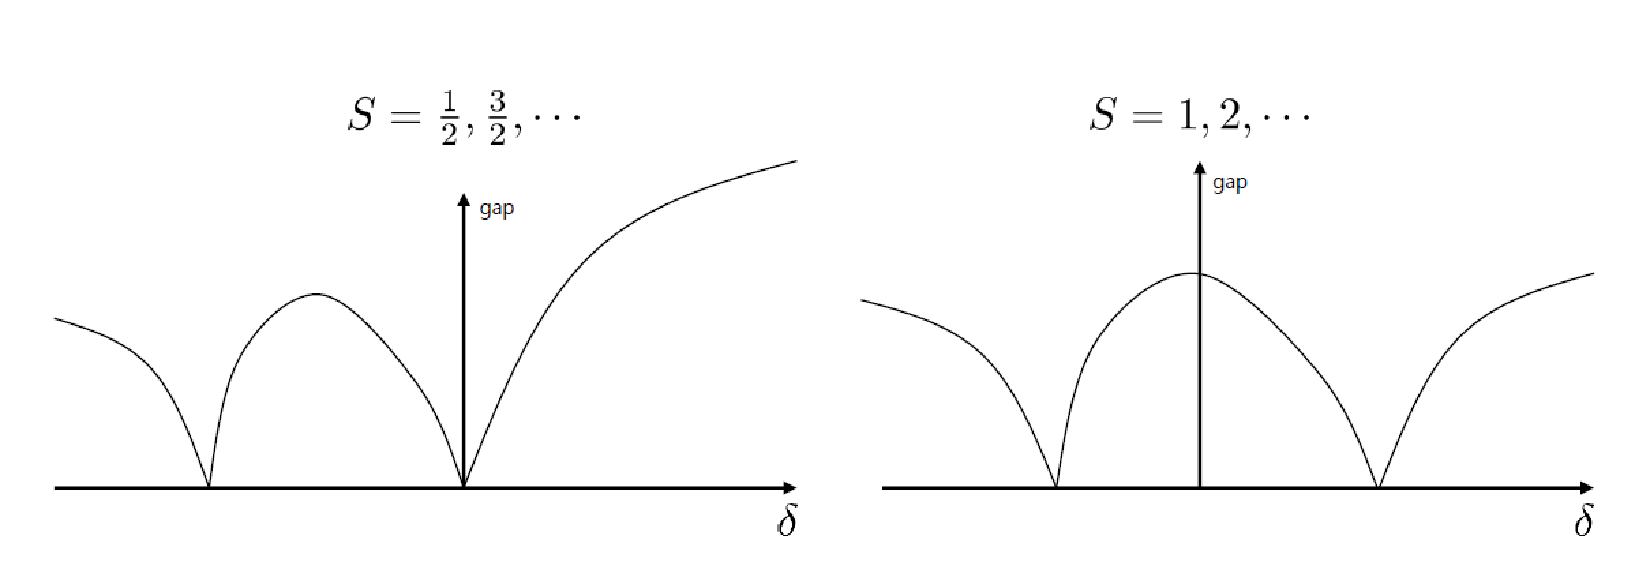
\includegraphics[width=0.9\textwidth]{graph_resize.pdf}
\caption{The gap of translation-broken Hamiltonian}
\end{figure}

Now we think the spin chain with magnetic field, whose Hamiltonian is
\begin{equation}
\mathcal{H}=J\sum(S_j^x S_{j+1}^x +S_j^y S_{j+1}^y + \Delta S_j^z S_{j+1}^z)-H\sum_j S_j^z
\end{equation}
This Hamiltonian still contains $U(1)$ symmetry and translational symmetry. Then we still have same analysis, except we may have $\langle S_j^z\rangle=m\neq 0$ possibly. Now since $-S_j^z=S-n_j$ where $n_j$ is the number of 'bosonic' particles, we have
\begin{equation}
m=\langle S_j^z\rangle=-S+\langle n_j\rangle
\end{equation}
thus $\langle n_j\rangle=S+m$. We often call $\langle n_j\rangle=\nu$ a "filling factor", because it represents how many particles are in one unit cell. From this we get the average density, $\rho_0=\frac{S+m}{a}$.

Lattice translation changes $\phi\mapsto \phi-\pi\rho_0 a=\phi-\pi(S+m)=\phi-\pi\nu$, thus
\begin{equation}
e^{2ip\phi}\mapsto e^{2ip\phi}e^{-2\pi i p\nu}
\end{equation}
Now we write down $\nu=p'/q'$ where $p',q'$ are coprimes. Then we can say that $e^{2ip\phi}$ is translation invariant only if $p=nq'$ for some $n\in \mathbb{Z}$, and all $e^{2ip\phi}$ with $p\neq nq'$ are forbidden.

Furthermore, considering the boundary condition $\phi\sim \phi+\pi$, if $\nu=p'/q'$, then $q'$ times of translation gives $\phi\mapsto \phi-\pi p'\sim \phi$. Thus with filling factor $\nu=p'/q'$, we may say that we have effectively $\mathbb{Z}/q'\mathbb{Z}$ symmetry. Mixing this with $U(1)$ symmetry, the system has $U(1)\times \mathbb{Z}/q'\mathbb{Z}$ symmetry. But if $q'$ is large enough, then we may consider $\mathbb{Z}/q'\mathbb{Z}$ as $U(1)$ group, and the symmetry becomes $U(1)\times U(1)$, which can be considered as the chiral symmetry.
\noindent\rule{\textwidth}{1pt}
\newline